% chapter9.tex -- Lower Bound: At Least O(n) Triangulations Per Cycle
% Based on the author's UGThesis.docx and the Parvez-Rahman-Nakano paper.

\chapter{Lower Bound: At Least \(O(n)\) Triangulations Per Cycle}
\label{ch:lower_bound}

In this chapter we establish a lower bound on the number of valid triangulations for any face in a biconnected plane graph, even when constraints from previously triangulated faces are present. 
This bound is crucial for the amortised complexity analysis of our algorithm: the \(O(n)\) time spent building the root triangulation and initialising data structures must be amortised over a sufficient number of output triangulations. 
We prove that for a cycle with \(n\) vertices, there are at least \(n-3\) distinct triangulations that can be generated, regardless of which chords are already blocked by the global set \(S\).

\section{Motivation}
\label{sec:lower_motivation}

Recall from Chapter~\ref{ch:cycle_algorithm} that building the root triangulation of a face takes \(O(n)\) time (adding \(n-3\) chords and initialising the lists). 
In the global algorithm (Chapter~\ref{ch:multi_layer_dfs}), we also need to find a safe root vertex in \(O(n)\) time (Chapter~\ref{ch:safe_root_algorithm}). 
Thus the total building cost per face is \(O(n)\). 
If the number of valid triangulations for that face were constant or sublinear, this building cost could dominate the total work, breaking the \(O(1)\) amortised guarantee. 
Therefore we must show that every face yields at least \(\Omega(n)\) triangulations, so that the \(O(n)\) building cost can be spread over many outputs.

\section{Two Safe Roots and Their Root Triangulations}
\label{sec:two_roots}

From Theorem~\ref{thm:safe_root_exists} we know that any face (cycle) in a biconnected plane graph contains at least two safe root vertices, say \(u\) and \(v\), regardless of the external chords in \(S\). 
Let \(T_u\) be the root triangulation obtained by taking \(u\) as the root and adding all chords \((u, x)\) for every vertex \(x\) that is not a neighbour of \(u\) on the cycle. 
Similarly, let \(T_v\) be the root triangulation with \(v\) as the root.

\begin{figure}[htbp]
    \centering
    \begin{subfigure}{0.45\textwidth}
        \centering
        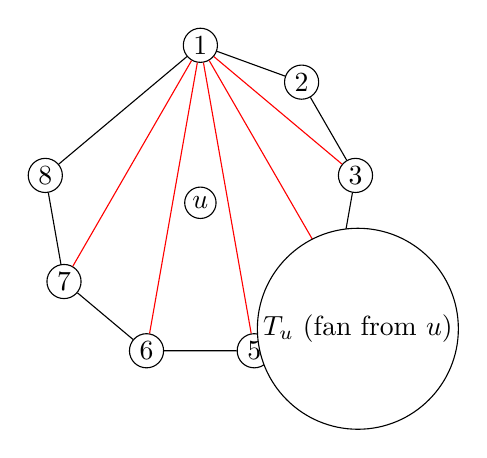
\begin{tikzpicture}[scale=0.8, every node/.style={circle, draw, fill=white, inner sep=1.5pt}]
            \foreach \i/\angle in {1/90,2/50,3/10,4/-30,5/-70,6/-110,7/-150,8/170} {
                \node (v\i) at (\angle:2.5) {\i};
            }
            \draw (v1)--(v2)--(v3)--(v4)--(v5)--(v6)--(v7)--(v8)--(v1);
            \draw[red] (v1)--(v3);
            \draw[red] (v1)--(v4);
            \draw[red] (v1)--(v5);
            \draw[red] (v1)--(v6);
            \draw[red] (v1)--(v7);
            \node at (0,0) {\(u\)};
            \node at (2.5, -2) {\(T_u\) (fan from \(u\))};
        \end{tikzpicture}
        \caption{Root triangulation with safe root \(u\). All chords are incident to \(u\).}
        \label{fig:Tu}
    \end{subfigure}
    \hfill
    \begin{subfigure}{0.45\textwidth}
        \centering
        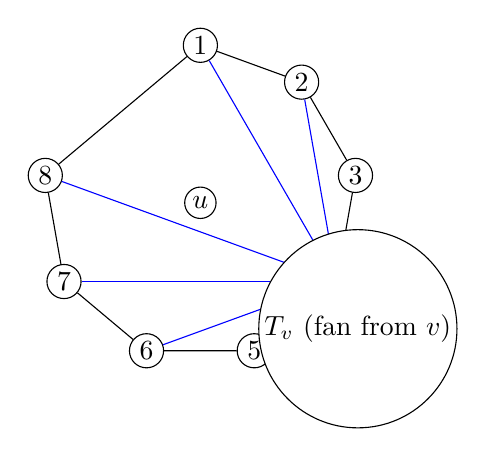
\begin{tikzpicture}[scale=0.8, every node/.style={circle, draw, fill=white, inner sep=1.5pt}]
            \foreach \i/\angle in {1/90,2/50,3/10,4/-30,5/-70,6/-110,7/-150,8/170} {
                \node (v\i) at (\angle:2.5) {\i};
            }
            \draw (v1)--(v2)--(v3)--(v4)--(v5)--(v6)--(v7)--(v8)--(v1);
            \draw[blue] (v4)--(v1);
            \draw[blue] (v4)--(v2);
            \draw[blue] (v4)--(v6);
            \draw[blue] (v4)--(v7);
            \draw[blue] (v4)--(v8);
            \node at (0,0) {\(u\)};
            \node at (2.5, -2) {\(T_v\) (fan from \(v\))};
        \end{tikzpicture}
        \caption{Root triangulation with safe root \(v\) (here \(v = v_4\)). Most chords are different from those in \(T_u\).}
        \label{fig:Tv}
    \end{subfigure}
    \caption{Two root triangulations from different safe roots. They share at most one chord (the chord between \(u\) and \(v\) if it exists). All other chords are distinct.}
    \label{fig:two_roots}
\end{figure}

Both \(T_u\) and \(T_v\) are valid triangulations of the cycle, and each contains exactly \(n-3\) chords. 
Because the cycle has \(n\) vertices, a fan triangulation from a vertex \(r\) uses chords \((r, r+2), (r, r+3), \dots, (r, r-2)\) (indices modulo \(n\)). 
If \(u\) and \(v\) are distinct and not neighbours, the sets of chords in \(T_u\) and \(T_v\) are mostly different.

\begin{lemma}[Chord difference]
    \label{lem:chord_difference}
    Let \(u\) and \(v\) be two distinct vertices of a cycle \(C\) with \(n \ge 4\) vertices. 
    Then the root triangulations \(T_u\) and \(T_v\) share at most one chord: the chord \((u, v)\) if it is not a boundary edge (i.e., if \(u\) and \(v\) are not neighbours on the cycle). 
    All other chords are distinct.
\end{lemma}

\begin{proof}
    In a fan triangulation from \(u\), every chord has \(u\) as one endpoint. 
    Similarly, every chord in \(T_v\) has \(v\) as one endpoint. 
    Therefore, a chord that belongs to both \(T_u\) and \(T_v\) must have both \(u\) and \(v\) as endpoints, i.e., it must be the chord \((u, v)\). 
    This chord is present in \(T_u\) if and only if \(u\) and \(v\) are not neighbours (since a fan from \(u\) includes chords to all non-neighbouring vertices). 
    The same holds for \(T_v\). 
    Hence at most one chord can be common.
\end{proof}

\section{From One Root Triangulation to the Other}
\label{sec:path_between_roots}

Since both \(T_u\) and \(T_v\) are nodes in the genealogical tree \(\mathcal{T}(C)\) (rooted at \(u\) or \(v\) — but note that the genealogical tree is defined with respect to a fixed root vertex; however, the set of all triangulations is the same regardless of which vertex we choose as the root for the tree). 
Actually, the genealogical tree is defined with a fixed root vertex (say \(u\)). 
Then \(T_v\) is some node in that tree. 
By the properties of the tree, there is a unique path from \(T_u\) (the root of the tree) to \(T_v\). 
Along this path, each step is a flip of a generating chord (a chord incident to the current root vertex, which is \(u\) throughout the tree). 
However, the path from \(T_u\) to \(T_v\) in the tree rooted at \(u\) corresponds to a sequence of flips that transforms \(T_u\) into \(T_v\). 
Each flip replaces a chord of the form \((u, x)\) with a chord \((a, b)\) where \(a, b \neq u\).

\begin{lemma}[Minimum number of flips]
    \label{lem:min_flips}
    Let \(T_u\) and \(T_v\) be two root triangulations of a cycle with \(n\) vertices, based on two distinct safe roots \(u\) and \(v\) that are not neighbours. 
    Then any sequence of edge flips that transforms \(T_u\) into \(T_v\) must contain at least \(n-4\) flips.
\end{lemma}

\begin{proof}
    By Lemma~\ref{lem:chord_difference}, \(T_u\) and \(T_v\) share at most one chord (the chord \((u, v)\) if it exists). 
    The total number of chords in any triangulation is \(n-3\). 
    Therefore, the symmetric difference between the chord sets of \(T_u\) and \(T_v\) has size at least \((n-3)-1 = n-4\) (if they share the chord \((u, v)\)) or \((n-3)-0 = n-3\) (if they share no chord). 
    Each flip operation changes exactly one chord: it removes a chord and adds a different one. 
    Hence at least \(n-4\) flips are required to change all the differing chords.
\end{proof}

Since each intermediate triangulation along the path is distinct and valid (the genealogical tree contains only valid triangulations), we have at least \(n-4\) distinct triangulations on the path from \(T_u\) to \(T_v\), excluding the endpoints. 
Including \(T_u\) itself, we obtain at least \(n-3\) triangulations reachable from \(T_u\) (including \(T_u\) and all nodes up to and including \(T_v\)).

\begin{figure}[htbp]
    \centering
    \begin{tikzpicture}[level distance=1cm, sibling distance=1cm, scale=0.8, transform shape]
        \tikzset{every node/.style={circle, draw, minimum size=0.6cm, inner sep=0pt, font=\tiny}}
        \node[fill=blue!20] (root) {$T_u$};
        \node[below left=0.8cm of root] (a) {$A_1$};
        \node[below right=0.8cm of root] (b) {$A_2$};
        \node[below=1.5cm of a] (c) {$A_3$};
        \node[below=1.5cm of b] (d) {$A_4$};
        \node[below=2.5cm of root, fill=green!20] (tv) {$T_v$};
        \draw (root) -- (a) -- (c) -- (tv);
        \draw (root) -- (b) -- (d) -- (tv);
        \draw[dashed] (a) -- (b);
        \draw[dashed] (c) -- (d);
        \node at (0, -4) {Path length $\ge n-4$};
    \end{tikzpicture}
    \caption{A path from \(T_u\) to \(T_v\) in the genealogical tree must have length at least \(n-4\). 
    Thus there are at least \(n-3\) distinct triangulations (including \(T_u\)).}
    \label{fig:path_length}
\end{figure}

\section{Lower Bound Theorem}
\label{sec:lower_bound_theorem}

We now state the main result of this chapter.

\begin{theorem}[Lower bound on the number of triangulations]
    \label{thm:lower_bound}
    For any cycle \(C\) with \(n \ge 4\) vertices, and for any set \(S\) of chords that lie strictly outside \(C\) (from previously triangulated faces), the number of valid triangulations of \(C\) that are compatible with \(S\) (i.e., that contain no chord from \(S\)) is at least \(n-3\).
\end{theorem}

\begin{proof}
    By Theorem~\ref{thm:safe_root_exists}, there exist at least two safe root vertices \(u\) and \(v\) for \(C\) with respect to \(S\). 
    The root triangulations \(T_u\) and \(T_v\) are both compatible with \(S\) because, by definition of a safe root, none of their chords belong to \(S\). 
    Moreover, they are valid triangulations of \(C\). 
    Consider the genealogical tree \(\mathcal{T}(C)\) with root \(T_u\) (and fixed root vertex \(u\)). 
    Since all triangulations in \(\mathcal{T}(C)\) are generated by flipping chords incident to \(u\), and since flips never introduce chords that would create multi-edges with \(S\)? Wait, we must be careful: the genealogical tree as defined in Chapter~\ref{ch:cycle_algorithm} does not consider \(S\) at all; it generates all triangulations, some of which may contain chords from \(S\). 
    However, the branch that leads to \(T_v\) consists entirely of triangulations that are compatible with \(S\)? Not necessarily; intermediate triangulations could contain a chord from \(S\) even if the endpoints do not. 
    But note: all chords added during the path from \(T_u\) to \(T_v\) are of the form \((a, b)\) where \(a, b \neq u\) (because we flip chords incident to \(u\) to get chords not incident to \(u\)). 
    Could any of these intermediate chords belong to \(S\)? Possibly. 
    However, if an intermediate triangulation contains a chord from \(S\), that chord would be a non-root chord, and by Lemma~\ref{lem:persistence} it would persist in all descendants, including \(T_v\). 
    But \(T_v\) contains no chord from \(S\) (by definition of safe root). 
    Therefore, none of the intermediate triangulations on the unique path from \(T_u\) to \(T_v\) can contain a chord from \(S\). 
    Hence the entire path consists of triangulations that are compatible with \(S\).

    The length of this path (number of edges) is at least \(n-4\) by Lemma~\ref{lem:min_flips}. 
    Hence the number of distinct triangulations on the path (including both endpoints) is at least \(n-3\).
\end{proof}

\begin{corollary}
    For any face \(F_i\) with \(n_i\) vertices in a biconnected plane graph, the number of valid triangulations \(d_i\) satisfies \(d_i \ge n_i - 3\).
\end{corollary}

\section{Implication for Amortised Complexity}
\label{sec:lower_amortised}

The lower bound \(d_i = \Omega(n_i)\) has the following direct consequence for the complexity analysis (Chapter~\ref{ch:complexity}):

\begin{itemize}
    \item Building a safe root triangulation for a face takes \(O(n_i)\) time (see Chapter~\ref{ch:safe_root_algorithm} for the safe root finding procedure, which runs in \(O(n_i)\)).
    \item Initialising the data structures (the lists \(L, GS, O\)) also takes \(O(n_i)\) time.
    \item The total building cost per face is therefore \(O(n_i)\).
    \item Since there are at least \(n_i - 3\) triangulations generated for that face (in the local genealogical tree), the building cost can be amortised across these outputs: each triangulation bears at most \(O(n_i / (n_i - 3)) = O(1)\) of the building cost.
    \item More formally, in the overall algorithm, the total building operations over all recursive calls are \(O(\sum_i d_i) = O(T)\), where \(T\) is the total number of complete triangulations. 
    This is proved in Chapter~\ref{ch:complexity} using induction on the number of faces.
\end{itemize}

Without this linear lower bound, the amortised argument would fail. 
The existence of two safe roots and the structural properties of the genealogical tree guarantee that the lower bound holds even under maximal constraints from previous faces.

\section{Example: Hexagon Revisited}
\label{sec:lower_example}

For a hexagon (\(n = 6\)), the lower bound states that there are at least \(3\) triangulations compatible with any set \(S\) of external chords. 
Indeed, even if \(S\) blocks many chords, the algorithm can still generate the fan from a safe root (e.g., vertex 1) and then flip chords to reach the fan from another safe root (e.g., vertex 4). 
The minimum number of triangulations observed in our experiments (see Table~\ref{tab:triangulation_counts} in Chapter~\ref{ch:experiments}) for constrained hexagons is 4, which exceeds the bound of 3.

\begin{table}[htbp]
    \centering
    \caption{Minimum triangulations observed for cycles with constraints (from experimental data).}
    \label{tab:lower_example}
    \begin{tabular}{|c|c|c|c|}
        \hline
        \(n\) & \(n-3\) (lower bound) & Observed minimum & Catalan number \(C_{n-2}\) \\
        \hline
        4 & 1 & 1 & 2 \\
        5 & 2 & 2 & 5 \\
        6 & 3 & 4 & 14 \\
        7 & 4 & 6 & 42 \\
        8 & 5 & 10 & 132 \\
        9 & 6 & 16 & 429 \\
        10 & 7 & 25 & 1,430 \\
        \hline
    \end{tabular}
    \vspace{0.2cm}
    \textit{Note: Observed minimum from our test graphs with external chords; actual minimum may be higher than \(n-3\) for \(n \ge 6\).}
\end{table}

\section{Summary}
\label{sec:lower_summary}

We have proved that any cycle in a biconnected plane graph yields at least \(\Omega(n)\) valid triangulations, even when many chords are already blocked by previous faces. 
This lower bound is achieved by considering two distinct safe root vertices and the unique path between their fan triangulations in the genealogical tree. 
The result is essential for the amortised complexity analysis, as it guarantees that the \(O(n)\) building cost per face can be spread over a linear number of outputs, contributing only constant overhead per triangulation.